%%%%%%%%%%%%%%%%%%%%%%%%%%%%%%%%%%%%%%%%%%%%%%%%%%%%%%%%%%
%% HEIG-VD / institut REDS
%%
%% Modèle Latex pour laboratoire
%% 
%% Fichiers à changer : 
%%            - constantes.tex
%%            - Tous les fichiers du corps du rapport 
%%
%% Auteur : MIM
%% Date   : 27.09.2017
%%%%%%%%%%%%%%%%%%%%%%%%%%%%%%%%%%%%%%%%%%%%%%%%%%%%%%%%%%

% Paramétrage du papier utilisé
\documentclass[a4paper,12pt,oneside]{article}

% Ne pas toucher, nécessaire à la mise en forme
\usepackage[utf8]{inputenc} 
\usepackage[T1]{fontenc} % Nouvelle norme pour codage des caractères
\usepackage{lmodern} % Nouvelle forme de la fonte ComputerModern
\usepackage[french]{babel} % Règles typographiques françaises, césures
\usepackage{graphicx} % Insertion images
\usepackage{epstopdf} % Convertir les images eps vers pdf
\epstopdfsetup{outdir=./Images/converted_to_pdf/} % Dossier de sortie des images converties
\pagenumbering{arabic}
\usepackage[top=3cm, bottom=3cm, left=3cm, right=3cm, showframe=false]{geometry}
\usepackage{amsmath}
\usepackage{hyperref}
\hypersetup{hidelinks} % pas d'encadrement rouge autour des liens
\addto\captionsfrench{\renewcommand{\tablename}{Tableau}} % "Tableau" au lieu de "Table"
\usepackage{pdfpages}
\usepackage{color}
\usepackage{float}
\usepackage{caption}
\usepackage{needspace}
\usepackage{tikz}
\usetikzlibrary{fit}

% \capture{fichier}{légende}{label}{contenu de remplacement}
% Insère images/<fichier>.png si l'image existe, sinon le contenu de
% remplacement (schéma TikZ) ou un cadre vide à compléter.
\newcommand{\capture}[4]{%
  \begin{figure}[H]
    \centering
    \IfFileExists{images/#1.png}{%
      \includegraphics[width=0.9\textwidth,height=0.5\textheight,keepaspectratio]{images/#1.png}}{%
    \IfFileExists{images/#1.jpg}{%
      \includegraphics[width=0.9\textwidth,height=0.6\textheight,keepaspectratio]{images/#1.jpg}}{%
      \if\relax\detokenize{#4}\relax
        \fbox{\parbox[c][4cm][c]{0.8\textwidth}{\centering\color{red}
          Capture à ajouter : \texttt{images/\detokenize{#1}.png}}}%
      \else
        \resizebox{\ifdim\width>\textwidth\textwidth\else\width\fi}{!}{#4}%
      \fi}}
    \caption{#2}
    \label{#3}
  \end{figure}}


% \extrait{fichier}{hauteur}{légende}{label} : extrait de schéma encadré et centré
\newcommand{\extrait}[4]{%
  \begin{figure}[H]
    \centering
    \setlength{\fboxsep}{4pt}\fbox{\includegraphics[height=#2,width=0.85\textwidth,keepaspectratio]{images/#1}}
    \caption{#3}
    \label{#4}
  \end{figure}}

% fichier avec les constantes (à adapter pour les étudiants)
%%%%%%%  Constantes %%%%%%%%

\newcommand{\nomAuteur}{M. Thiébaud}

\newcommand{\titre}{Registre à décalage - Chenillard}

\newcommand{\nbrlabo}{4} % numéro de laboratoire

\newcommand{\prof}{E. Messerli}

\newcommand{\assistant}{Y. Graf}

\newcommand{\classe}{SysLog1}

\newcommand{\departement}{Technologies industrielles (TIN)}

\newcommand{\cours}{Systèmes Logiques 1 (SysLog1)}


% Entête et pieds de page (A ADAPTER)
\pagestyle{empty}
\usepackage{fancyhdr}
\setlength{\headheight}{27.06pt}
\pagestyle{fancy}
% Entête :
\renewcommand{\headrulewidth}{1pt}
\fancyhead[L]{Labo\nbrlabo: \titre} 
\fancyhead[R]{Rapport de laboratoire} 
% Pied de page
\fancyfoot{} % clear all footer fields
\renewcommand{\footrulewidth}{1pt}
\fancyfoot[R]{Page \thepage} 
\fancyfoot[L]{HEIG-VD | \nomAuteur }

% debut du corps du rapport 
\begin{document}	
	% première page
	%%%%%%%%%%%%%%%%%%%%%%%%%%%%%%%%%%%%%%%%%%%%%%%%%%%%%%%%
% Ce document ne doit pas être modifié
% Il faut modifier les informations depuis le fichier
% constantes.tex
%%%%%%%%%%%%%%%%%%%%%%%%%%%%%%%%%%%%%%%%%%%%%%%%%%%%%%%%



\begin{center}

\includegraphics[height=2cm]{./images/logo_heig.pdf}
\hfill 
\includegraphics[height=2cm]{./images/logo_hesso.pdf}
\end{center}

\vfill

\begin{center}
	\Large Laboratoire \nbrlabo:\\
	\huge \titre \\
\end{center}


\begin{center}
	\begin{tabular}{l l}
		Département:          & \departement\\
		Unité d'enseignement: & \cours\\
	\end{tabular}
\end{center}


\vfill

%\begin{center}
%	\includegraphics{Images/it.png}
%\end{center}

\vfill

\begin{tabular}{l l}
	\Large	Auteur:    			  & \Large \nomAuteur\\
	Professeur:           & \prof\\
	Assistant:			  & \assistant\\
	Classe:               & \classe\\
	Date:                 & \today\\
\end{tabular}

\vfill

\begin{center}

\includegraphics[height=1.5cm]{./images/logo_reds.pdf}
\end{center}
	% enlève le numero sur la premiere page
	\thispagestyle{empty}
	\setcounter{page}{1}
	\newpage

	% table des matières
	\pagenumbering{roman}
	\tableofcontents
	\clearpage

	% tables des figures et des tableaux
	\listoffigures
	\listoftables
	\clearpage

	% retour à la numérotation normale pour le corps du rapport
	\pagenumbering{arabic}

	% ici débute le corps du rapport
	% changer les sections au cas par cas afin de vous adapter au maximum aux critères
	%\section{Introduction}
	%\section{Analyse et conception}
	%\section{Réalisation et implémentation}
	%\section{Simulation}
	%\section{Conclusion}
	% les méthodologies présentée ci-dessus est une bonne approche pour les petits projets qui ne demandent pas beaucoup de documentation mais n'est pas adaptée à des gros projets où plusieurs personnes vont rédiger de la documentation (Utilisation de git)
	% En modifiant les documents depuis deux endroits différents, si vous répartissez le travail par "thème", chacun va modifier un document et à la fin il suffira de merge ensemble les changements
	\section{Introduction}

Ce laboratoire consiste à concevoir dans Logisim un registre à décalage 4 bits, puis un registre 8 bits avec chargement parallèle et décalage à droite ou à gauche, et enfin un chenillard sur 8 LED. Le chenillard est ensuite testé sur la carte MAX\_V\_\allowbreak 80P\_25P.

	\section{Analyse et conception}

\subsection{Partie 1 : registre à décalage à droite 4 bits}

Si \texttt{en\_sh\_i} = 1, le registre se décale à droite à chaque flanc montant de l'horloge et \texttt{ser\_r\_i} entre en $Q_3$. Sinon, il garde son état. Chaque cellule est donc une bascule D précédée d'un multiplexeur qui choisit entre maintien (entrée 0, sa propre sortie) et décalage (entrée 1, la sortie de la cellule voisine). Le reset est asynchrone et agit directement sur les bascules.

\extrait{circ_p1_cellule.png}{3cm}{Une cellule du registre 4 bits : multiplexeur et bascule D}{fig:circ_p1_cellule}

\subsection{Partie 2 : registre 8 bits avec chargement et décalage}

Le registre a trois fonctions synchrones, par ordre de priorité : chargement, décalage (à droite ou à gauche) et maintien. Le tableau~\ref{tab:fct_sync} donne l'état futur $Q^+$ du registre au prochain flanc montant de \texttt{clock\_i}, en fonction des entrées de commande. Le reset n'y figure pas car il est asynchrone : tant que \texttt{reset\_i} = 1, le registre vaut 00000000, quelles que soient l'horloge et les autres entrées.

\begin{table}[H]
  \centering
  \small
  \begin{tabular}{c c c l c}
    \hline
    \texttt{load\_i} & \texttt{en\_sh\_i} & \texttt{Right\_nLeft\_i} & \textbf{Fonction} & $Q^+_7 \dots Q^+_0$ \\
    \hline
    1 & - & - & Chargement parallèle & \texttt{val\_i(7..0)} \\
    0 & 1 & 1 & Décalage à droite    & \texttt{ser\_r\_i}, $Q_7 \dots Q_1$ \\
    0 & 1 & 0 & Décalage à gauche    & $Q_6 \dots Q_0$, \texttt{ser\_l\_i} \\
    0 & 0 & - & Maintien             & $Q_7 \dots Q_0$ \\
    \hline
  \end{tabular}
  \caption{Table des fonctions synchrones de \texttt{srg8\_ld\_sh} (\texttt{-} : valeur indifférente)}
  \label{tab:fct_sync}
\end{table}

\texttt{load\_i} n'est soumis à aucune autre condition : le chargement l'emporte donc sur le décalage. \texttt{Right\_nLeft\_i} n'est pris en compte que si \texttt{en\_sh\_i} = 1. Cette table se traduit directement par trois multiplexeurs 8 bits en cascade placés devant le registre :
\begin{itemize}
  \item le premier (\texttt{Right\_nLeft\_i}) choisit entre la valeur décalée à droite et celle décalée à gauche ;
  \item le deuxième (\texttt{en\_sh\_i}) choisit entre cette valeur décalée et l'état actuel (maintien) ;
  \item le dernier (\texttt{load\_i}) impose \texttt{val\_i}, ce qui rend le chargement prioritaire.
\end{itemize}
Le reset asynchrone passe avant tout. L'entrée WE du registre est fixée à 1.

\extrait{circ_p2_mux.png}{4cm}{Chaîne de multiplexeurs devant le registre 8 bits}{fig:circ_p2_mux}

\subsection{Partie 3 : chenillard}

Le chenillard fait tourner le pattern de manière cyclique : le bit qui sort d'un côté du registre doit rentrer de l'autre. Pour cela, $Q_0$ est rebouclé sur \texttt{ser\_r\_i} (rotation à droite) et $Q_7$ sur \texttt{ser\_l\_i} (rotation à gauche). Une porte NOT convertit \texttt{nReset\_i}, actif bas, en reset actif haut pour le registre.

\extrait{circ_p3_rebouclage.png}{5cm}{Rebouclage de $Q_0$ et $Q_7$ sur les entrées série}{fig:circ_p3_rebouclage}

	\section{Réalisation}

Les trois circuits ont été réalisés dans le fichier \texttt{srg8\_ld\_sh.circ}, dans les circuits préparés par la donnée.

\subsection{Registre 4 bits \texttt{srg4\_sh\_r}}

Les quatre cellules sont chaînées de gauche à droite : la première reçoit \texttt{ser\_r\_i}, et chacune des suivantes reçoit la sortie de sa voisine. L'enable, l'horloge et le reset sont communs aux quatre bascules. Un splitter regroupe les sorties dans le bus \texttt{reg\_o}, avec la cellule d'entrée sur le bit 3.

\capture{p1_schema}{Schéma Logisim du registre 4 bits \texttt{srg4\_sh\_r}}{fig:p1_schema}{}

\subsection{Registre 8 bits \texttt{srg8\_ld\_sh}}

Les valeurs décalées sont obtenues sans logique, par simple recâblage des bits avec des splitters. Pour le décalage à droite, chaque bit $i$ reçoit $Q_{i+1}$ et le bit 7 reçoit \texttt{ser\_r\_i}. Pour le décalage à gauche, chaque bit $i$ reçoit $Q_{i-1}$ et le bit 0 reçoit \texttt{ser\_l\_i}. La sortie du registre revient aussi sur l'entrée 0 du multiplexeur d'enable pour le maintien.

\capture{p2_schema}{Schéma Logisim du registre 8 bits \texttt{srg8\_ld\_sh}}{fig:p2_schema}{}

\subsection{Chenillard}

Le chenillard instancie \texttt{srg8\_ld\_sh} sans le modifier. Les entrées de commande sont reliées directement, \texttt{pattern\_i} va sur \texttt{val\_i}, et la sortie \texttt{reg\_o} pilote les LED. Un splitter extrait $Q_0$ et $Q_7$ de la sortie pour les reboucler sur les entrées série.

\capture{p3_schema}{Schéma Logisim du \texttt{chenillard}}{fig:p3_schema}{}

	\newpage
\section{Simulation}

Chaque partie a été simulée manuellement sur Logisim dans le but de visualiser les priorités et les rebouclages des systèmes.
\subsection{Partie 1 : registre 4 bits}

Le tableau~\ref{tab:p1_tests} donne, pour chaque flanc montant de
\texttt{clock\_sti}, la fonction testée et la valeur attendue sur \texttt{reg\_obs}.
Les valeurs observées sur le chronogramme (figure~\ref{fig:p1_chrono})
correspondent toutes aux valeurs attendues.

\begin{table}[H]
  \centering
  \small
  \begin{tabular}{c l c}
    \hline
    \textbf{Flanc} & \textbf{Fonction testée} & \textbf{\texttt{reg\_obs} attendu} \\
    \hline
    15 et 25~µs & \textbf{Reset prioritaire} (\texttt{en\_sh} = \texttt{ser\_r} = 1) & \texttt{0000} \\
    35~µs  & Décalage à droite, \texttt{ser\_r\_sti} = 1 & \texttt{1000} \\
    45~µs  & Décalage à droite, \texttt{ser\_r\_sti} = 1 & \texttt{1100} \\
    55~µs  & Décalage à droite, \texttt{ser\_r\_sti} = 1 & \texttt{1110} \\
    65~µs  & Décalage à droite, \texttt{ser\_r\_sti} = 1 & \texttt{1111} \\
    75 et 85~µs & Maintien (\texttt{en\_sh\_sti} = 0)   & \texttt{1111} \\
    95~µs  & Décalage à droite, \texttt{ser\_r\_sti} = 0 & \texttt{0111} \\
    105~µs & Décalage à droite, \texttt{ser\_r\_sti} = 0 & \texttt{0011} \\
    110~µs & \textbf{Reset asynchrone} & \texttt{0000} \\
    \hline
  \end{tabular}
  \caption{Tests de simulation de \texttt{srg4\_sh\_r}}
  \label{tab:p1_tests}
\end{table}

\capture{p1_chrono_annote}{Chronogramme de \texttt{srg4\_sh\_r\_sim}}{fig:p1_chrono}{}

\needspace{12\baselineskip}
\subsection{Partie 2 : registre 8 bits}

Le tableau~\ref{tab:p2_tests} donne, pour chaque flanc montant de
\texttt{clock\_i}, la fonction testée et la valeur attendue sur \texttt{reg\_o}.
Les valeurs observées sur le chronogramme (figures~\ref{fig:p2_chrono_a} et~\ref{fig:p2_chrono_b})
correspondent toutes aux valeurs attendues.

\begin{table}[H]
  \centering
  \begin{tabular}{c l c}
    \hline
    \textbf{Flanc} & \textbf{Fonction testée} & \textbf{\texttt{reg\_o} attendu} \\
    \hline
    55~µs  & Chargement de \texttt{10110010}                    & \texttt{1011 0010} \\
    85~µs  & Maintien (\texttt{en\_sh\_i} = 0)                  & \texttt{1011 0010} \\
    105~µs & Décalage à droite, \texttt{ser\_r\_i} = 0          & \texttt{0101 1001} \\
    120~µs & Décalage à droite, \texttt{ser\_r\_i} = 1          & \texttt{1010 1100} \\
    130~µs & Décalage à gauche, \texttt{ser\_l\_i} = 1          & \texttt{0101 1001} \\
    140~µs & Décalage à gauche, \texttt{ser\_l\_i} = 0          & \texttt{1011 0010} \\
    150~µs & \textbf{Load prioritaire sur le décalage} (\texttt{11110000}) & \texttt{1111 0000} \\
    165~µs & Décalage à droite, \texttt{ser\_r\_i} = 1          & \texttt{1111 1000} \\
    175~µs & Décalage à droite, \texttt{ser\_r\_i} = 1          & \texttt{1111 1100} \\
    185~µs & \textbf{Reset asynchrone}      & \texttt{0000 0000} \\
    \hline
  \end{tabular}
  \caption{Tests de simulation de \texttt{srg8\_ld\_sh}}
  \label{tab:p2_tests}
\end{table}

\capture{p2_chrono_a}{Chronogramme de \texttt{srg8\_ld\_sh\_sim} (1/2) : de 0 à 108~µs}{fig:p2_chrono_a}{}
\capture{p2_chrono_b}{Chronogramme de \texttt{srg8\_ld\_sh\_sim} (2/2) : de 103 à 200~µs}{fig:p2_chrono_b}{}

\needspace{12\baselineskip}
\subsection{Partie 3 : chenillard}

Le tableau~\ref{tab:p3_tests} donne, pour chaque flanc montant de
\texttt{clock\_i}, la fonction testée et la valeur attendue sur \texttt{LED\_out}.
Les valeurs observées sur le chronogramme (figures~\ref{fig:p3_chrono_a} et~\ref{fig:p3_chrono_b})
correspondent toutes aux valeurs attendues.

\begin{table}[H]
  \centering
  \small
  \begin{tabular}{c l c}
    \hline
    \textbf{Flanc} & \textbf{Fonction testée} & \textbf{\texttt{LED\_out} attendu} \\
    \hline
    5~µs   & Reset actif (\texttt{nReset\_i} = 0)               & \texttt{0000 0000} \\
    30~µs  & Chargement du pattern \texttt{10000000}            & \texttt{1000 0000} \\
    50~µs  & Maintien (\texttt{enable\_i} = 0)                  & \texttt{1000 0000} \\
    65 à 125~µs      & Rotation à droite (7 flancs)                       & \texttt{0100 0000} $\rightarrow$ \texttt{0000 0001} \\
    135~µs & \textbf{Rebouclage à droite} & \texttt{1000 0000} \\
    145~µs & \textbf{Rebouclage à gauche} & \texttt{0000 0001} \\
    155 et 165~µs     & Rotation à gauche                                  & \texttt{0000 0010}, \texttt{0000 0100} \\
    175~µs & Maintien (\texttt{enable\_i} = 0)                  & \texttt{0000 0100} \\
    185~µs & \textbf{Load prioritaire} (\texttt{11010000}) & \texttt{1101 0000} \\
    200 à 230~µs     & Rotation à droite            & \texttt{0110 1000} $\rightarrow$ \texttt{0000 1101} \\
    240~µs & Rebouclage avec plusieurs bits actifs              & \texttt{1000 0110} \\
    255~µs & Changement de sens (gauche)                        & \texttt{0000 1101} \\
    260~µs & \textbf{Reset asynchrone}      & \texttt{0000 0000} \\
    \hline
  \end{tabular}
  \caption{Tests de simulation du chenillard}
  \label{tab:p3_tests}
\end{table}

\capture{p3_chrono_a}{Chronogramme de \texttt{chenillard\_sim} (1/2) : de 0 à 138~µs}{fig:p3_chrono_a}{}
\capture{p3_chrono_b}{Chronogramme de \texttt{chenillard\_sim} (2/2) : de 132 à 266~µs}{fig:p3_chrono_b}{}

    \section{Intégration et test}

Le circuit \texttt{main} a été intégré sur la carte MAX\_V\_CONSOLE avec le menu \og FPGA \fg{}. Il a ensuite été programmé dans la CPLD de la carte MAX\_V\_80P\_25P. Le test a été fait avec une horloge de 1 à 4~Hz fournie par la boîte de commande : chargement d'un pattern, rotation dans les deux sens, arrêt et reset.

\begin{figure}[H]
  \centering
  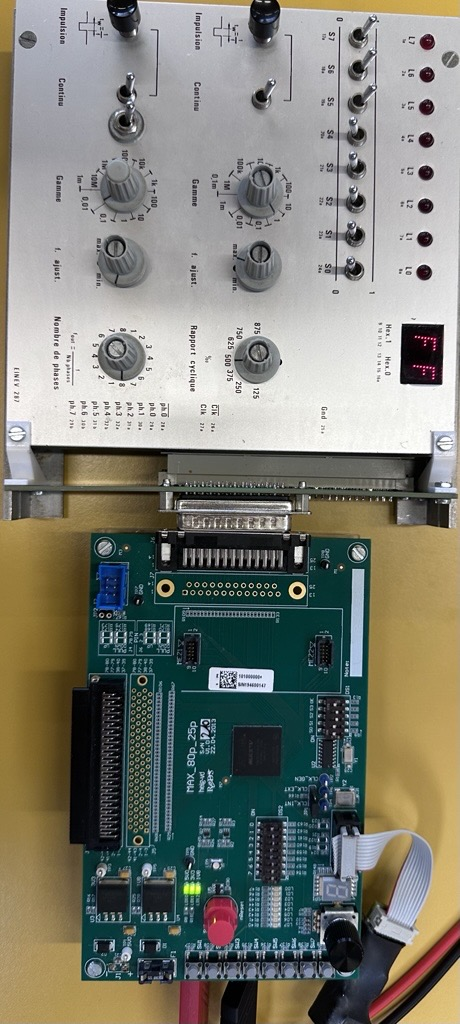
\includegraphics[angle=90,width=0.75\textwidth]{images/p3_carte.jpg}
  \caption{Test du chenillard sur la carte MAX\_V\_80P\_25P et la console}
  \label{fig:p3_carte}
\end{figure}

\textbf{Validation :} montage validé par M. Graf le 27.11.2026.
    
	\section{Conclusion}

Les trois circuits ont été vérifiés en simulation, et le chenillard fonctionne sur la carte. Pour obtenir la rotation, il a suffi de reboucler les sorties extrêmes du registre sur ses entrées série, sans modifier le registre lui-même.

Les simulations ont aussi confirmé l'ordre des priorités. Le reset est le plus prioritaire : il est asynchrone et remet le registre à zéro immédiatement, sans attendre de flanc d'horloge et quelles que soient les autres entrées. Vient ensuite le chargement parallèle (\texttt{load}), qui l'emporte sur le décalage ou la rotation même lorsque l'enable est actif. Enfin, si ni le reset, ni le load, ni l'enable ne sont actifs, le registre conserve sa valeur.

	
	%Section pour la signature
	\needspace{7\baselineskip}
	\section{Signatures}
  
    Yverdon-les-Bains le \today \\

	\vspace{1cm}
	\noindent\hfill
	\begin{tabular}{@{}p{0.45\textwidth}@{}}
	  \rule{\linewidth}{0.4pt} \\
	   M. Thiébaud
	\end{tabular}
  

	% si des annexes sont nécessaires ajouter :
	% \section{Annexes}
	% Changement de notation en lettre : 
	%\appendix
	% insertion d'une nouvelle page
	%\newpage
	% Ajouter un fichier latec dans le fichier courant
	%\input{Chapitres/cdc.tex}
	
%Fin du document
\end{document}


